\documentclass[journal,10pt,a4paper]{IEEEtran}
\usepackage[spanish,es-nodecimaldot,es-noshorthands,es-tabla]{babel}
\usepackage{amsmath,amssymb}
\usepackage{newtxmath}
\usepackage{fontspec}
\setmainfont{texgyretermes}[Extension=.otf,UprightFont=*-regular,BoldFont=*-bold,ItalicFont=*-italic,BoldItalicFont=*-bolditalic]
\usepackage{graphicx}
\usepackage{booktabs}
\usepackage{siunitx}
\usepackage{cite}
\usepackage{url}
\sisetup{output-decimal-marker={.}, group-digits=false}
\graphicspath{{../A/resultados/1/}{../A/resultados/3/}{../figuras/}}

\begin{document}

\title{Caracterización Experimental y Modelado de Primer Orden de un Motor de Corriente Continua para el Accionamiento en Azimut de un Telescopio}

\author{Ignacio~Vargas~Fernández, Athina~Salim, Francesca~Giavarini y~Tiziano~De~Marco%
\thanks{Trabajo Práctico N.\textsuperscript{o}~2, IOR442 Sistemas de Control, Universidad de San Andrés.}}

\markboth{IOR442 Sistemas de Control --- Trabajo Práctico N.\textsuperscript{o}~2}{}

\maketitle

\begin{abstract}
Se presenta la etapa inicial de la identificación de un motor de corriente continua destinado al accionamiento del eje de azimut de un telescopio. A partir de un ensayo de diez ciclos de seis escalones de ciclo de trabajo (\emph{duty}) comprendidos entre 0.60 y 0.75, registrado a \SI{1}{kHz} y suavizado mediante un promedio móvil causal de \SI{0.1}{s}, se caracteriza la respuesta de velocidad. Se muestra que el transitorio frente a un escalón es monótono y compatible con un sistema de primer orden de constante de tiempo cercana a \SI{110}{ms}, una vez descontado el retardo introducido por el filtro. La relación estática entre velocidad y \emph{duty} se aproxima por la recta $\omega_{ss}=245.9\,d-134.9$~rad/s, con coeficiente de determinación $R^2=0.996$. Se interpreta físicamente el modelo propuesto $\dot\omega=-p(\omega-\omega_{ref})+pK_{dc}(d-d_{ref})$, se deducen su equilibrio y su forma equivalente $\dot\omega+p\omega=bd+c$, y se implementa y verifica su integración por el método de Euler explícito. Se documentan además dos fenómenos que el modelo de primer orden no describe: un rizado periódico al doble de la frecuencia de giro y una deriva lenta de la velocidad de régimen a lo largo del ensayo.
\end{abstract}

\begin{IEEEkeywords}
Motor de corriente continua, identificación de sistemas, modelo de primer orden, promedio móvil, método de Euler, PWM.
\end{IEEEkeywords}

\section{Introducción}
\IEEEPARstart{E}{l} diseño de un sistema de control por realimentación de estados exige disponer, en primer término, de un modelo dinámico de la planta que sea a la vez sencillo y fiel en la región de operación de interés~\cite{ogata,franklin,astrom}. En el caso del accionamiento en azimut de un telescopio, la planta es un motor de corriente continua alimentado mediante modulación por ancho de pulso (PWM), cuya velocidad angular debe describirse en función del ciclo de trabajo aplicado. El modelo que resulte de esta etapa constituirá la base para el diseño de los controladores de posición lento y rápido que se abordan en la Parte~B del trabajo.

La identificación a partir de datos experimentales~\cite{ljung} comprende varias etapas: la inspección de los registros, la selección de una estructura de modelo, la estimación de sus parámetros y la validación con datos no utilizados en el ajuste. El presente informe aborda las tres primeras de manera preparatoria: (i)~el análisis exploratorio del ensayo, que justifica la estructura de primer orden y provee estimaciones preliminares de sus parámetros; (ii)~la interpretación física del modelo propuesto por la cátedra; y (iii)~la implementación y verificación del integrador numérico con el que se calculará la respuesta del modelo durante la estimación por mínimos cuadrados no lineales.

El resto del trabajo se organiza como sigue. La Sección~\ref{sec:exp} describe el ensayo y los datos. La Sección~\ref{sec:a1} presenta el análisis de los registros. La Sección~\ref{sec:a2} desarrolla el modelo propuesto. La Sección~\ref{sec:a3} trata su integración numérica. La Sección~\ref{sec:disc} discute las implicancias para la identificación y la Sección~\ref{sec:conc} resume las conclusiones.

\section{Dispositivo experimental y datos}\label{sec:exp}
El ensayo se realizó en un banco de pruebas en el que un microcontrolador ESP32 generó la señal PWM y registró la posición angular del eje mediante un sensor magnético AS5600. La velocidad se obtuvo por diferenciación de la posición y se suavizó con un promedio móvil causal de duración $T_v=\SI{0.1}{s}$. El archivo provisto contiene \num{360060} muestras de tres señales: tiempo, \emph{duty} efectivo $d[k]$ y velocidad promediada $\omega_m[k]$.

El análisis de la señal de tiempo confirma un período de muestreo uniforme $T_s=\SI{1}{ms}$ (desviaciones menores que \SI{e-10}{s}). La entrada presenta 60 tramos de duración idéntica, \SI{6.001}{s}, que conforman diez ciclos de \SI{36}{s} con la secuencia comandada 0.65, 0.70, 0.75, 0.70, 0.65, 0.60. Los valores efectivos registrados son $d\in\{0.6000,\ 0.6510,\ 0.7020,\ 0.7490\}$, que corresponden exactamente a $153/255$, $166/255$, $179/255$ y $191/255$; es decir, el PWM posee una resolución de 8~bits y el valor aplicado es el entero más cercano al comandado. Por esta razón se emplea en todos los cálculos el \emph{duty} efectivo y no el nominal. Los siete primeros ciclos (\SIrange{0}{252}{s}) se reservan para el ajuste de parámetros y los tres restantes (\SIrange{252}{360}{s}) para la validación.

\section{Análisis de los datos experimentales}\label{sec:a1}

\subsection{Visión general del ensayo}
La Fig.~\ref{fig:completo} muestra la entrada y la velocidad durante todo el ensayo; la línea discontinua separa los tramos de ajuste y de validación. La Fig.~\ref{fig:ciclo} presenta en detalle el segundo ciclo, elegido para evitar el arranque del registro, en el que la velocidad parte de \SI{12.6}{rad/s} con $d=0.651$ y aún no se encuentra en régimen. Se aprecia a simple vista que la velocidad sigue fielmente la forma escalonada de la entrada, que cada nivel de \emph{duty} se corresponde con un nivel de velocidad bien definido (de unos \SI{13}{rad/s} para $d=0.60$ a unos \SI{50}{rad/s} para $d=0.75$) y que los niveles se alcanzan en una fracción pequeña de los \SI{6}{s} de cada tramo. Dos características merecen, sin embargo, atención: una oscilación de amplitud cercana a \SI{2}{rad/s} pico a pico superpuesta a cada nivel y un lento crecimiento de los niveles a lo largo de los diez ciclos.

\begin{figure*}[!t]
\centering
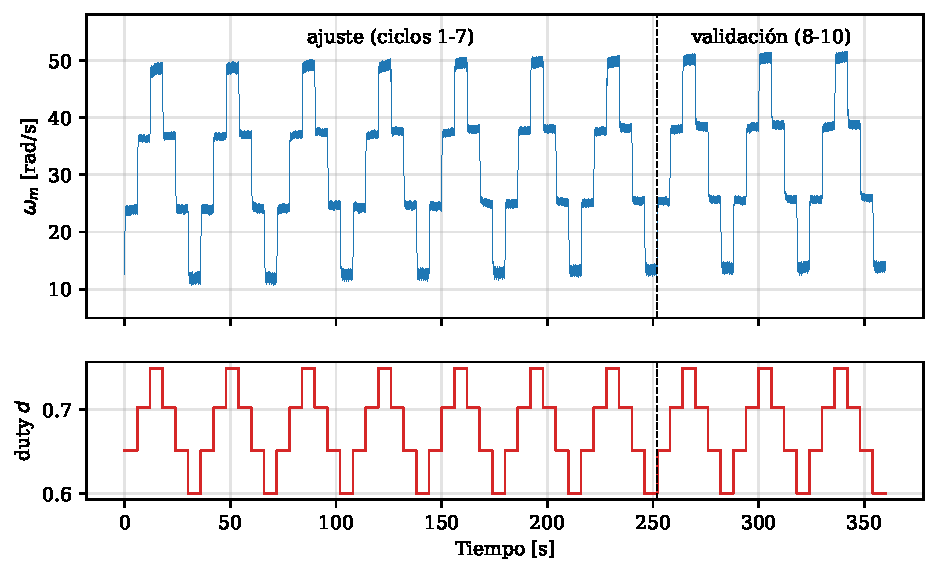
\includegraphics[width=0.85\textwidth]{fig_A1a_ensayo_completo.pdf}
\caption{Ensayo completo. Arriba: velocidad medida promediada $\omega_m$. Abajo: \emph{duty} efectivo. La línea discontinua en $t=\SI{252}{s}$ separa los siete ciclos de ajuste de los tres de validación.}
\label{fig:completo}
\end{figure*}

\begin{figure}[!t]
\centering
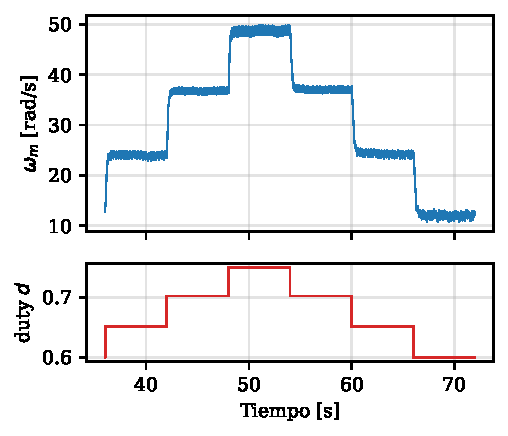
\includegraphics[width=\columnwidth]{fig_A1a_un_ciclo.pdf}
\caption{Detalle del segundo ciclo ($36\le t<\SI{72}{s}$): secuencia de seis escalones de \emph{duty} y velocidad resultante.}
\label{fig:ciclo}
\end{figure}

\subsection{Respuesta transitoria ante escalones}\label{sec:transitorio}
La velocidad no alcanza instantáneamente el nuevo nivel tras un cambio de \emph{duty}: aparece un transitorio de aproximadamente \SIrange{0.4}{0.5}{s}. El panel izquierdo de la Fig.~\ref{fig:escalon} muestra el escalón $0.651\rightarrow0.702$ en $t=\SI{42}{s}$. La respuesta es monótona y tiende exponencialmente al nuevo valor, sin oscilaciones propias de un par de polos complejos; las pequeñas excursiones por encima del valor final coinciden en forma y amplitud con el rizado presente antes del escalón, por lo que no constituyen un sobrepico dinámico. Este comportamiento es característico de un sistema de \emph{primer orden}.

Debe observarse, no obstante, que la curva medida arranca con pendiente prácticamente nula durante los primeros \SI{50}{ms}, lo que podría sugerir a primera vista un sistema de orden superior. Este efecto se explica por el promedio móvil: si la velocidad real es $\omega(t)=\omega_0+\Delta\omega(1-e^{-t/\tau})$, su promedio sobre la ventana precedente de longitud $T_v$ crece inicialmente en forma cuadrática, y su retardo medio respecto de la señal original es $T_v/2=\SI{50}{ms}$. Por ello, el instante en que la señal medida alcanza el 63.2\,\% del salto ($t_{63}=\SI{158}{ms}$ en promedio sobre los 59 escalones) sobreestima la constante de tiempo.

Para obtener una estimación consistente se ajustó, para cada uno de los 59 escalones, la constante $\tau$ de una respuesta normalizada de primer orden \emph{a la que se aplicó el mismo promedio móvil} que a los datos. Se obtuvo una mediana $\tau=\SI{110}{ms}$ (media \SI{108}{ms}, desvío \SI{28}{ms}), es decir, un polo preliminar $p\approx1/\tau\approx\SI{9.1}{s^{-1}}$. La curva de trazo discontinuo de la Fig.~\ref{fig:escalon} reproduce adecuadamente tanto la forma inicial como la aproximación al régimen. El panel derecho, que superpone las 59 respuestas normalizadas, revela una asimetría: los escalones de subida son más rápidos ($\bar\tau=\SI{82}{ms}$) que los de bajada ($\bar\tau=\SI{133}{ms}$). Un modelo lineal con un único polo no puede representar exactamente esta diferencia.

\begin{figure*}[!t]
\centering
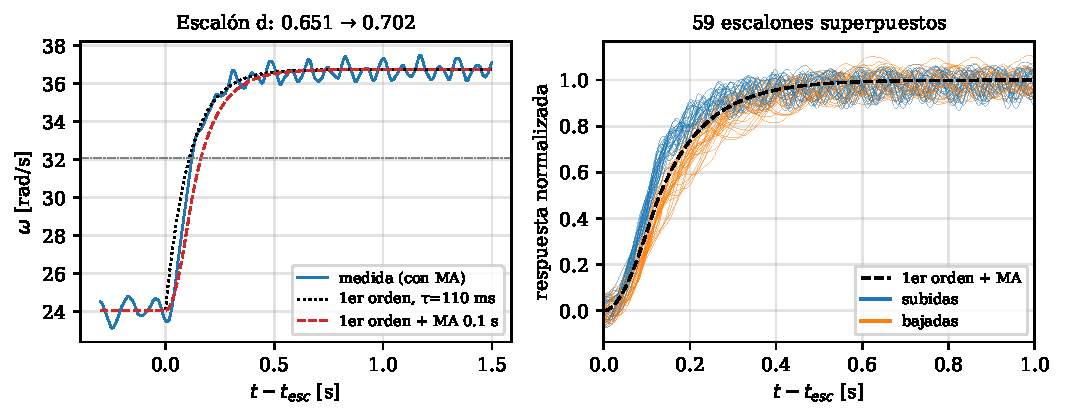
\includegraphics[width=0.9\textwidth]{fig_A1b_detalle_escalon.pdf}
\caption{Izquierda: escalón $d:0.651\rightarrow0.702$ en $t=\SI{42}{s}$, junto con una respuesta de primer orden de $\tau=\SI{110}{ms}$ sin filtrar (punteada) y filtrada con el promedio móvil de \SI{0.1}{s} (discontinua); la línea horizontal marca el 63.2\,\% del salto. Derecha: respuestas normalizadas $(\omega-\omega_0)/(\omega_1-\omega_0)$ de los 59 escalones del ensayo, distinguiendo subidas y bajadas.}
\label{fig:escalon}
\end{figure*}

El rizado observado en régimen fue analizado mediante la transformada de Fourier del último tramo de \SI{5}{s} de cada nivel. La Tabla~\ref{tab:rizado} muestra que su frecuencia dominante es, en todos los niveles, el doble de la frecuencia de rotación $\omega/2\pi$. Se trata, por lo tanto, de una perturbación \emph{sincrónica con el ángulo del eje} y no de una dinámica del motor; su origen más probable es un error dependiente del ángulo en la medición magnética (desalineación o inclinación del imán respecto del AS5600) o un par periódico de origen mecánico. Este rizado, de unos \SIrange{1.5}{2.5}{rad/s} pico a pico, no forma parte de la dinámica que describe un modelo de primer orden.

\begin{table}[!t]
\centering
\caption{Frecuencia dominante del rizado en régimen (ciclo 2)}
\label{tab:rizado}
\setlength{\tabcolsep}{4pt}
\begin{tabular}{cccc}
\toprule
$\bar\omega$ [rad/s] & $f_{giro}=\bar\omega/2\pi$ [Hz] & $f_{rizado}$ [Hz] & Pico a pico [rad/s]\\
\midrule
11.9 & 1.90 & 3.80 & 2.50\\
24.0 & 3.82 & 7.60 & 2.06\\
36.6 & 5.83 & 11.60 & 1.54\\
48.7 & 7.75 & 15.60 & 2.29\\
\bottomrule
\end{tabular}
\end{table}

\subsection{Característica estática velocidad--\emph{duty}}\label{sec:estatica}
Para cada uno de los 60 tramos se estimó la velocidad de régimen permanente $\omega_{ss}$ promediando las \num{1000} muestras de su último segundo. Puesto que el transitorio se extingue en menos de \SI{0.5}{s} (unas cinco constantes de tiempo), dicho intervalo, situado entre \SI{5}{s} y \SI{6}{s} después de cada cambio, está libre de efectos dinámicos; además, al abarcar varios períodos del rizado, el promedio lo atenúa eficazmente. Sobre los 60 pares $(d,\omega_{ss})$ se ajustó por mínimos cuadrados la recta
\begin{equation}
\omega_{ss}\approx m\,d+q,\qquad m=\SI{245.9}{rad/s},\quad q=\SI{-134.9}{rad/s},
\label{eq:recta}
\end{equation}
con coeficiente de determinación $R^2=0.9963$, error cuadrático medio de \SI{0.72}{rad/s} y residuo máximo de \SI{1.5}{rad/s}. La pendiente $m$ indica que la velocidad estacionaria aumenta \SI{2.46}{rad/s} por cada centésima de \emph{duty}. La Fig.~\ref{fig:estatica} muestra los puntos, coloreados según el ciclo, la recta ajustada y los residuos.

\begin{figure}[!t]
\centering
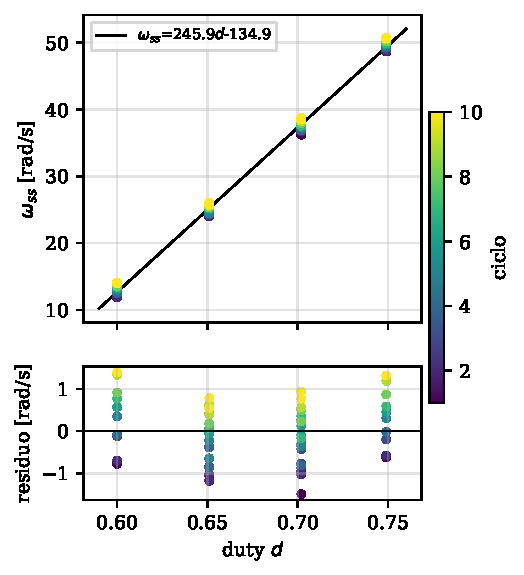
\includegraphics[width=0.92\columnwidth]{fig_A1c_regimen_permanente.pdf}
\caption{Velocidad de régimen de cada tramo en función del \emph{duty} (color: número de ciclo), recta de mínimos cuadrados~\eqref{eq:recta} y residuos.}
\label{fig:estatica}
\end{figure}

La adecuación de la aproximación lineal se juzga a partir de la estructura de los residuos (Tabla~\ref{tab:niveles}). Existe una leve curvatura: los residuos medios por nivel son positivos en los extremos y negativos en el centro, y las pendientes entre niveles consecutivos crecen de \num{234.7} a \num{255.7}~rad/s, es decir, se apartan de $m$ en menos de un 5\,\%. Sin embargo, esta curvatura (residuos medios de \SIrange{0.1}{0.4}{rad/s}) es menor que la dispersión de un mismo nivel entre ciclos (desvío de \SIrange{0.66}{0.77}{rad/s}), que domina claramente los residuos, como evidencia la estratificación por color de la Fig.~\ref{fig:estatica}. En consecuencia, la relación lineal es una aproximación adecuada en el intervalo ensayado $0.60\le d\le0.75$. No debe, en cambio, extrapolarse: la recta se anula en $d_0=-q/m=0.548$, valor que debe interpretarse como un indicador del umbral por debajo del cual el rozamiento seco detiene el motor, región que el ensayo evitó deliberadamente.

\begin{table}[!t]
\centering
\caption{Velocidad de régimen por nivel de \emph{duty}}
\label{tab:niveles}
\setlength{\tabcolsep}{4pt}
\begin{tabular}{ccccc}
\toprule
$d$ & Tramos & $\bar\omega_{ss}$ [rad/s] & Desvío [rad/s] & Residuo medio [rad/s]\\
\midrule
0.6000 & 10 & 13.05 & 0.77 & $+0.36$\\
0.6510 & 20 & 25.01 & 0.66 & $-0.21$\\
0.7020 & 20 & 37.63 & 0.71 & $-0.13$\\
0.7490 & 10 & 49.66 & 0.69 & $+0.33$\\
\bottomrule
\end{tabular}
\end{table}

La dispersión entre ciclos no es aleatoria. La velocidad de régimen media de cada ciclo crece en forma monótona desde \SI{30.31}{rad/s} en el primero hasta \SI{32.29}{rad/s} en el décimo, una deriva de unos \SI{2}{rad/s} (6.5\,\%) en seis minutos. La hipótesis más plausible es térmica: el calentamiento del motor y de sus cojinetes reduce la viscosidad del lubricante y, con ella, el rozamiento.

\section{Modelo dinámico propuesto}\label{sec:a2}

\subsection{Estructura y significado de los parámetros}
Se propone describir la dinámica de velocidad mediante
\begin{equation}
\dot\omega=-p\,(\omega-\omega_{ref})+p\,K_{dc}\,(d-d_{ref}),\qquad d_{ref}=0.675.
\label{eq:modelo}
\end{equation}
Esta estructura se justifica a partir de las ecuaciones del motor de corriente continua~\cite{franklin}. Con $J$ la inercia, $B$ el coeficiente de rozamiento viscoso, $T_f$ un par resistente aproximadamente constante (rozamiento seco~\cite{armstrong}), $R$ la resistencia de armadura, $K_t$ y $K_e$ las constantes de par y de fuerza contraelectromotriz, y $V_s$ la tensión de alimentación, de modo que la tensión media aplicada es $V=dV_s$, se tiene
\begin{align}
J\dot\omega&=K_t\,i-B\,\omega-T_f,\\
L\,\tfrac{di}{dt}&=dV_s-R\,i-K_e\,\omega.
\end{align}
Si la constante de tiempo eléctrica $L/R$ es despreciable frente a la mecánica, $i\approx(dV_s-K_e\omega)/R$ y resulta
\begin{equation}
\dot\omega=-\underbrace{\frac{B+K_tK_e/R}{J}}_{p}\,\omega+\underbrace{\frac{K_tV_s}{RJ}}_{b}\,d\;\underbrace{-\;\frac{T_f}{J}}_{c},
\label{eq:fisico}
\end{equation}
que es precisamente un sistema de primer orden afín en la entrada, de la misma forma que~\eqref{eq:modelo}. A la luz de~\eqref{eq:fisico}, los parámetros admiten la siguiente interpretación:
\begin{itemize}
\item $p$ [\si{s^{-1}}]: polo del sistema, cambiado de signo; su inversa $\tau=1/p$ es la constante de tiempo mecánica. Reúne el amortiguamiento viscoso y el electromagnético (fuerza contraelectromotriz) referidos a la inercia, y determina la rapidez de la respuesta.
\item $K_{dc}$ [(rad/s)/\emph{duty}, es decir \si{rad/s} por unidad de ciclo de trabajo, adimensional]: ganancia estática, igual a la variación de la velocidad de equilibrio por unidad de variación de \emph{duty}; físicamente, $K_{dc}=b/p=K_tV_s/(RB+K_tK_e)$.
\item $\omega_{ref}$ [\si{rad/s}]: velocidad de equilibrio cuando $d=d_{ref}$; fija el punto de operación nominal alrededor del cual se linealiza.
\item $d_{ref}$ [adimensional]: \emph{duty} de referencia, fijado en el centro del intervalo ensayado; no se estima.
\end{itemize}
La parametrización centrada en $d_{ref}$ tiene una ventaja práctica para la estimación: puesto que $d$ toma valores lejanos al origen, en la forma $bd+c$ los parámetros $b$ y $c$ estarían fuertemente correlacionados, mientras que $\omega_{ref}$ y $K_{dc}$ son prácticamente independientes y tienen un significado inmediato.

\subsection{Velocidad de equilibrio}
Para un \emph{duty} constante $d$, el equilibrio se obtiene imponiendo $\dot\omega=0$ en~\eqref{eq:modelo}. Si $p\neq0$,
\begin{equation}
\omega^*=\omega_{ref}+K_{dc}\,(d-d_{ref}).
\label{eq:equilibrio}
\end{equation}
Con $p>0$ el equilibrio es asintóticamente estable y la velocidad converge a él como $\omega(t)=\omega^*+(\omega(0)-\omega^*)e^{-pt}$. La expresión~\eqref{eq:equilibrio} es una recta en $d$ que coincide con la característica estática~\eqref{eq:recta} si $K_{dc}=m$ y $\omega_{ref}-K_{dc}d_{ref}=q$. El análisis de la Sección~\ref{sec:a1} provee entonces estimaciones preliminares: $K_{dc}\approx\SI{245.9}{rad/s}$, $\omega_{ref}\approx m\,d_{ref}+q=\SI{31.1}{rad/s}$ y, de los escalones, $p\approx\SI{9.1}{s^{-1}}$.

\subsection{Forma estándar}
Distribuyendo en~\eqref{eq:modelo},
\begin{equation}
\dot\omega+p\,\omega=\underbrace{p\,K_{dc}}_{b}\,d+\underbrace{p\,(\omega_{ref}-K_{dc}\,d_{ref})}_{c},
\label{eq:estandar}
\end{equation}
de donde
\begin{equation}
b=p\,K_{dc}\quad[\si{rad/s^2}],\qquad c=p\,(\omega_{ref}-K_{dc}\,d_{ref})\quad[\si{rad/s^2}].
\end{equation}
Nótese que $c/p=q$: el término independiente de la recta estática, negativo, se asocia según~\eqref{eq:fisico} al par de rozamiento seco $T_f=-Jc>0$. Con los valores preliminares, $b\approx\SI{2.24e3}{rad/s^2}$ y $c\approx\SI{-1.23e3}{rad/s^2}$.

\section{Integración numérica del modelo}\label{sec:a3}

\subsection{Discretización por Euler explícito}
La respuesta del modelo a la secuencia medida $d[k]$ se calcula integrando~\eqref{eq:modelo} con el método de Euler hacia adelante~\cite{butcher} y paso $\Delta t=T_s=\SI{1}{ms}$, igual al de muestreo, lo que permite usar directamente cada muestra de la entrada:
\begin{align}
\dot\omega[k]&=-p\,(\omega[k]-\omega_{ref})+p\,K_{dc}\,(d[k]-d_{ref}),\label{eq:wdot}\\
\omega[k+1]&=\omega[k]+\Delta t\,\dot\omega[k],\qquad \omega[0]=\omega_0.\label{eq:euler}
\end{align}
Reordenando,
\begin{equation}
\omega[k+1]=(1-p\Delta t)\,\omega[k]+p\Delta t\,\bigl[\omega_{ref}+K_{dc}(d[k]-d_{ref})\bigr],
\end{equation}
un sistema discreto de primer orden con polo $z_E=1-p\Delta t$, que aproxima al polo exacto $z=e^{-p\Delta t}$ con un error de orden $(p\Delta t)^2/2$. Se desprenden tres propiedades útiles: (i)~el esquema es estable si $|1-p\Delta t|<1$, es decir, $p<2/\Delta t=\SI{2000}{s^{-1}}$, condición holgadamente satisfecha para los valores de $p$ de interés; (ii)~para $p\approx\SI{9}{s^{-1}}$ resulta $p\Delta t\approx0.009$, por lo que el error de discretización es despreciable frente al ruido de medición; y (iii)~el punto fijo de~\eqref{eq:euler} cumple $\dot\omega[k]=0$, de modo que el método conserva exactamente el equilibrio~\eqref{eq:equilibrio} y, con él, la ganancia estática.

\subsection{Implementación}
La función \texttt{calcular\_velocidad} del código de la cátedra recibe el vector de parámetros $(K_{dc},\omega_{ref},p)$, la secuencia de \emph{duty} y la velocidad inicial, y devuelve un vector del mismo largo que la entrada, cuya primera muestra es la velocidad inicial. Dado que cada muestra depende de la anterior, la recursión~\eqref{eq:euler} se implementa con un lazo explícito; para los \num{252000} puntos del tramo de ajuste su ejecución demanda unos \SI{60}{ms}.

\subsection{Verificación}
Se verificó la implementación con los parámetros de prueba $K_{dc}=240$~(rad/s)/\emph{duty}, $\omega_{ref}=\SI{30}{rad/s}$, $p=\SI{8}{s^{-1}}$ y $d_{ref}=0.675$, un \emph{duty} constante $d=0.70$ y una velocidad inicial de \SI{30}{rad/s}, durante \SI{2}{s}. Por~\eqref{eq:equilibrio}, la velocidad de equilibrio analítica es
\begin{equation}
\omega^*=30+240\,(0.70-0.675)=\SI{36}{rad/s},
\end{equation}
y la solución exacta es $\omega(t)=36-6\,e^{-8t}$~rad/s, con $\tau=\SI{125}{ms}$ y un tiempo de establecimiento al 2\,\% de $4\tau=\SI{0.5}{s}$. La Fig.~\ref{fig:euler} muestra que la velocidad calculada converge al valor analítico; la Tabla~\ref{tab:euler} resume la comparación cuantitativa. La velocidad final difiere de $\omega^*$ en \SI{6.4e-7}{rad/s}, valor que coincide con el remanente esperado $6\,(1-p\Delta t)^{1999}$ del transitorio. La máxima discrepancia con la solución exacta, \SI{8.9}{mrad/s} (0.15\,\% del salto), se produce en torno a $t=\tau$ y es positiva, ya que $z_E<e^{-p\Delta t}$ hace que Euler responda ligeramente más rápido que el sistema continuo.

\begin{figure}[!t]
\centering
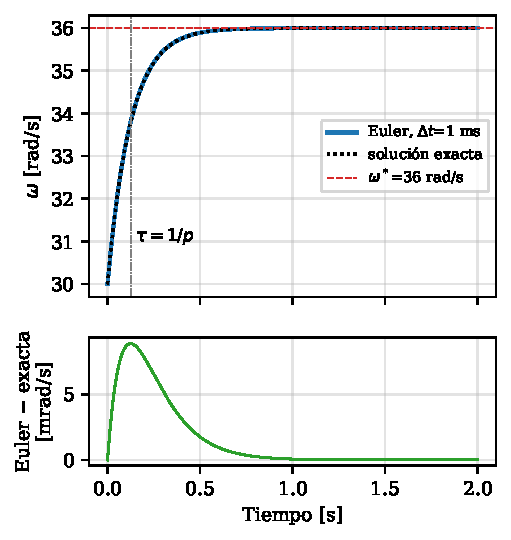
\includegraphics[width=0.92\columnwidth]{fig_A3c_verificacion_euler.pdf}
\caption{Verificación del integrador con los parámetros de prueba ($d=0.70$, $\omega_0=\SI{30}{rad/s}$). Arriba: solución por Euler, solución exacta y equilibrio analítico. Abajo: diferencia entre ambas soluciones.}
\label{fig:euler}
\end{figure}

\begin{table}[!t]
\centering
\caption{Verificación del integrador de Euler}
\label{tab:euler}
\begin{tabular}{lc}
\toprule
Magnitud & Valor\\
\midrule
Equilibrio analítico $\omega^*$ & \SI{36.000000}{rad/s}\\
Euler en $t=\SI{2}{s}$ & \SI{35.999999}{rad/s}\\
Error final & \SI{-6.4e-7}{rad/s}\\
Máx.\ $|\omega_E-\omega_{exacta}|$ & \SI{8.9e-3}{rad/s}\\
Polo discreto Euler / exacto & 0.99200 / 0.99203\\
\bottomrule
\end{tabular}
\end{table}

\section{Discusión}\label{sec:disc}
La estructura de primer orden está respaldada por la forma monótona de los 59 transitorios y por la linealidad de la característica estática en el intervalo ensayado; ambos hechos son coherentes con el modelo físico~\eqref{eq:fisico} cuando la dinámica eléctrica es rápida frente a la mecánica.

El análisis reveló, sin embargo, tres apartamientos respecto de ese comportamiento ideal. El primero es un rizado de amplitud aproximadamente constante, sincrónico con el ángulo del eje, cuya frecuencia es el doble de la de giro. El segundo es una asimetría entre los transitorios de subida y de bajada, propia de un comportamiento no lineal que podría atribuirse al rozamiento~\cite{armstrong} o al modo de conducción del puente que alimenta el motor. El tercero es una deriva lenta y monótona de la velocidad de régimen a lo largo del ensayo. Ninguno de ellos está contemplado en el modelo~\eqref{eq:modelo}, y conviene tenerlos presentes al interpretar cualquier comparación entre el modelo y las mediciones.

\section{Conclusiones}\label{sec:conc}
Se analizó un ensayo escalonado de un motor de corriente continua accionado por PWM. La respuesta de velocidad presenta un transitorio de primer orden con constante de tiempo cercana a \SI{110}{ms}, una vez tenido en cuenta el retardo de \SI{50}{ms} que introduce el promedio móvil, y una característica estática lineal $\omega_{ss}=245.9\,d-134.9$~rad/s con $R^2=0.996$ en el intervalo $0.60\le d\le0.75$. Se interpretaron físicamente los parámetros del modelo propuesto, se dedujeron su equilibrio $\omega^*=\omega_{ref}+K_{dc}(d-d_{ref})$ y los coeficientes $b=pK_{dc}$ y $c=p(\omega_{ref}-K_{dc}d_{ref})$, y se obtuvieron estimaciones preliminares $K_{dc}\approx\SI{246}{rad/s}$, $\omega_{ref}\approx\SI{31.1}{rad/s}$ y $p\approx\SI{9.1}{s^{-1}}$. Se implementó la integración por Euler con paso de \SI{1}{ms} y se verificó que converge al equilibrio analítico de \SI{36}{rad/s} con un error inferior a \SI{e-6}{rad/s}. Se documentaron, por último, un rizado sincrónico con la rotación, una asimetría entre transitorios de subida y de bajada y una deriva lenta de la velocidad de régimen, fenómenos que el modelo de primer orden no describe.

\appendices
\section{Entorno de software}
Los cálculos se realizaron con Python~3.13.7, NumPy~2.4.3, SciPy~1.17.1 y Matplotlib~3.10.9. El archivo \texttt{parte\_A\_ej1\_a\_3.py} genera todas las figuras y valores numéricos de este informe (ejecución: \texttt{python parte\_A\_ej1\_a\_3.py datos\_motor.csv}); la función \texttt{calcular\_velocidad} se encuentra en \texttt{script\_identificacion.py}.

\begin{thebibliography}{9}
\bibitem{ogata}
K.~Ogata, \emph{Modern Control Engineering}, 5th~ed. Upper Saddle River, NJ: Prentice Hall, 2010.

\bibitem{franklin}
G.~F. Franklin, J.~D. Powell y A.~Emami-Naeini, \emph{Feedback Control of Dynamic Systems}, 6th~ed. Upper Saddle River, NJ: Pearson, 2010.

\bibitem{ljung}
L.~Ljung, \emph{System Identification: Theory for the User}, 2nd~ed. Upper Saddle River, NJ: Prentice Hall, 1999.

\bibitem{butcher}
J.~C. Butcher, \emph{Numerical Methods for Ordinary Differential Equations}, 2nd~ed. Chichester: Wiley, 2008.

\bibitem{astrom}
K.~J. {\AA}str{\"o}m y R.~M. Murray, \emph{Feedback Systems: An Introduction for Scientists and Engineers}. Princeton, NJ: Princeton University Press, 2008.

\bibitem{armstrong}
B.~Armstrong-H{\'e}louvry, P.~Dupont y C.~Canudas de Wit, ``A survey of models, analysis tools and compensation methods for the control of machines with friction,'' \emph{Automatica}, vol.~30, no.~7, pp.~1083--1138, 1994.
\end{thebibliography}

\end{document}
